\margininbox{Bivi}{
     \begin{itemize}
    \item Rhys Tyers
    \item Clare Tan
    \end{itemize}}{\explo}


\section{A rather cold welcome}

When Rhys Tyers and Clare Tan flew out a week before the main 2014 expedition, they had no inkling that the Hollow Mountain reserved a rather unpleasant welcome for them both, for after a long ascent through whirling milky white clouds and dense, cold and drippy dwarf pine they broke onto a bleak landscape. The sun had not started to pierce through the shifting cloud cover, giving the place a desolate, empty look. Less empty however was the bivi shakehole, which the wan light barely touched: \bignote{a large snow plug occupied the space which was to be filled with the buzz and bustle of excitement only a score of like-minded explorers can produce}.

This was rather problematic since it kept the bivi temperature far below that the plateau --- at the best of times, the bivi shakehole is a couple of degrees cooler than elsewhere --- prevented the access to the stone circle, rendered the usual washing space impracticable and finally because the melt runoff kept mixing with years of bivi sedimentation, the result of which was a most repugnant mixture.

As the main core of the expedition arrived however, large numbers of helping hands, adequate job division and most of all, a determination to vanquish the uninvited iceberg saw a large operation of snow removal take place. Some was hauled out of the shakehole and dumped into \passage{M10} --- maybe a fraction resisted further melting and was later hauled up for drinking water the following year--- another portion sawed off and sculpted and one particularly large lump provided shelf space for the drying dishes and cutlery.

Little by little, the ice receded and the cold bivi nights turned more pleasant, even as news of further underground discoveries came floating back from the plateau. The weather improved gradually, and it was not without a pinch of sadness that we saw the last of it meekly retreating below the scree under a hot summer's afternoon.

\name{Tanguy Racine}

\begin{pagefigure}
\checkoddpage \ifoddpage \forcerectofloat \else \forceversofloat \fi
   \centering

       \begin{subfigure}[t]{0.393\textwidth}
        \centering
        \frame{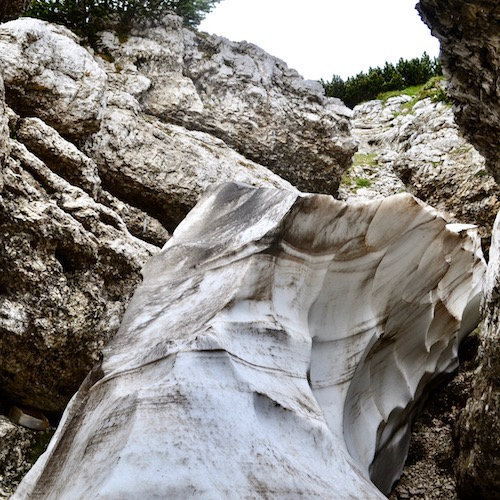
\includegraphics[width=\linewidth]{images/2014/welcome-2014/dsc_1239.jpg}}
        \caption{} \label{Snow plug}
    \end{subfigure}
    \hfill
     \begin{subfigure}[t]{0.59\textwidth}
        \centering
        \frame{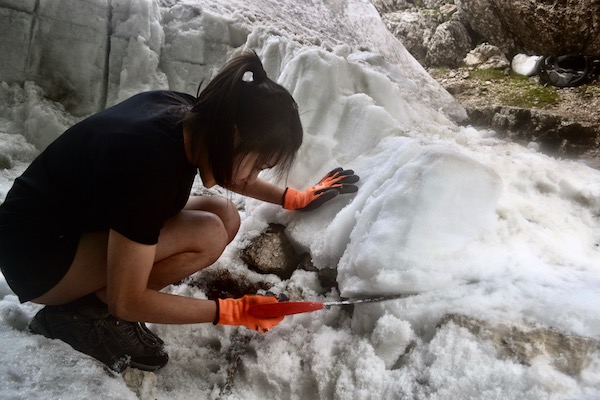
\includegraphics[width=\linewidth]{images/2014/welcome-2014/dsc_1333.jpg}}
        \caption{} \label{Snow sawing}
    \end{subfigure}
    
    \vspace{0cm}
    \centering
    \begin{subfigure}[t]{0.59\textwidth}
        \centering
        \frame{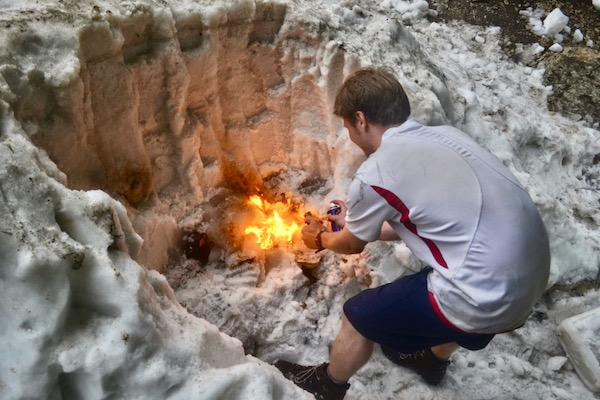
\includegraphics[width=\linewidth]{images/2014/welcome-2014/dsc_1324.jpg}}
        \caption{} \label{Snow burning}
    \end{subfigure}
    \hfill
    \begin{subfigure}[t]{0.393\textwidth}
        \centering
        \frame{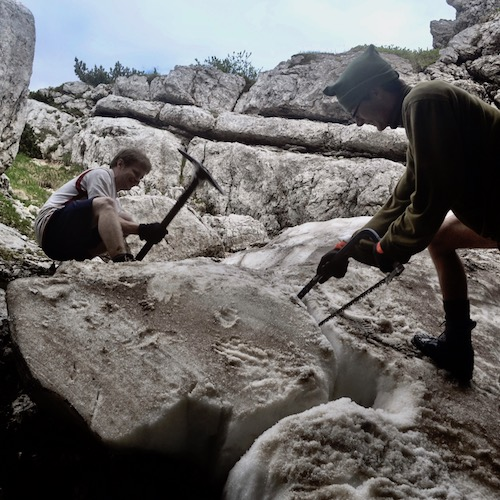
\includegraphics[width=\linewidth]{images/2014/welcome-2014/dsc_1327.jpg}}
        \caption{} \label{Snow carving}
    \end{subfigure}

    \vspace{0cm}
    \begin{subfigure}[t]{\textwidth}
    \centering
        \frame{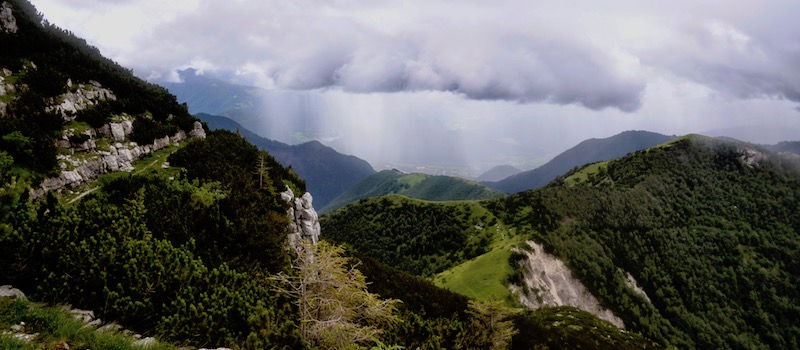
\includegraphics[width=\linewidth]{images/2014/welcome-2014/dsc_1252.jpg}}
        \caption{} \label{Panorama from mule path}
    \end{subfigure}
    \caption{
    \emph{(a)} The snow plug at the back of the bivi
    \emph{(b)} Sarah, cutting away of block of snow to uncover a stone seat
    \emph{(c)} Will French burning away at the iceberg.
    \emph{(d)} Carving, sawing and hacking at the edges of the snow plug
    \emph{(e)} On the mule path looking back towards Tolmin and the Soa valley. --- Rhys Tyers}
\end{pagefigure}
